\documentclass[11pt, a4paper, twoside]{article}   	% use "amsart" instead of "article" for AMSLaTeX format

\usepackage{geometry}                		% See geometry.pdf to learn the layout options. There are lots.
\usepackage{pdfpages}
\usepackage{caption}
\usepackage{minted}
\usepackage[german]{babel}			% this end the next are needed for german umlaute
\usepackage[utf8]{inputenc}
\usepackage{color}
\usepackage{graphicx}
\usepackage{titlesec}
\usepackage{fancyhdr}
\usepackage{lastpage}
\usepackage{hyperref}
\usepackage[autostyle=false, style=english]{csquotes}
\usepackage{mathtools}
\usepackage{tabularx}
% http://www.artofproblemsolving.com/wiki/index.php/LaTeX:Symbols#Operators
% =============================================
% Layout & Colors
% =============================================
\geometry{
   a4paper,
   total={210mm,297mm},
   left=20mm,
   right=20mm,
   top=20mm,
   bottom=30mm
 }	

\definecolor{myred}{rgb}{0.8,0,0}
\definecolor{mygreen}{rgb}{0,0.6,0}
\definecolor{mygray}{rgb}{0.5,0.5,0.5}
\definecolor{mymauve}{rgb}{0.58,0,0.82}

\setcounter{secnumdepth}{4}


% the default java directory structure and the main packages
\newcommand{\srcDir}{../src/ImageJ/plugins/bva2}
\newcommand{\imageDir}{images}


% =============================================
% Code Settings
% =============================================
\newenvironment{code}{\captionsetup{type=listing}}{}
\newmintedfile[javaFile]{java}{
	linenos=true, 
	frame=single, 
	breaklines=true, 
	tabsize=2,
	numbersep=5pt,
	xleftmargin=10pt,
	baselinestretch=1,
	fontsize=\footnotesize
}

\newmintinline[inlineJava]{java}{}
\newminted[javaSource]{java}{
	breaklines=true, 
	tabsize=2,
	autogobble=true,
	breakautoindent=false
}


\newcommand{\xvdash}[1]{%
  \vdash^{\mkern-10mu\scriptscriptstyle\rule[-.9ex]{0pt}{0pt}#1}%
}

% =============================================
% Page Style, Footers & Headers, Title
% =============================================
\title{Übung 6}
\author{Gattringer Marko, Ruhsam Christoph}

\lhead{Gattringer Marko, Ruhsam Christoph}
\chead{BVA}
\rhead{Übung 6}

\lfoot{S1810454012, S1810454036}
\cfoot{}
\rfoot{ \thepage / \pageref{LastPage} }
\renewcommand{\footrulewidth}{0.4pt}
% =============================================
% D O C U M E N T     C O N T E N T
% =============================================
% =============================================
% 2016.10.13: 1 
% 2016.10.14: 2
% =============================================
\pagestyle{fancy}
\begin{document}
\setlength{\headheight}{15mm}
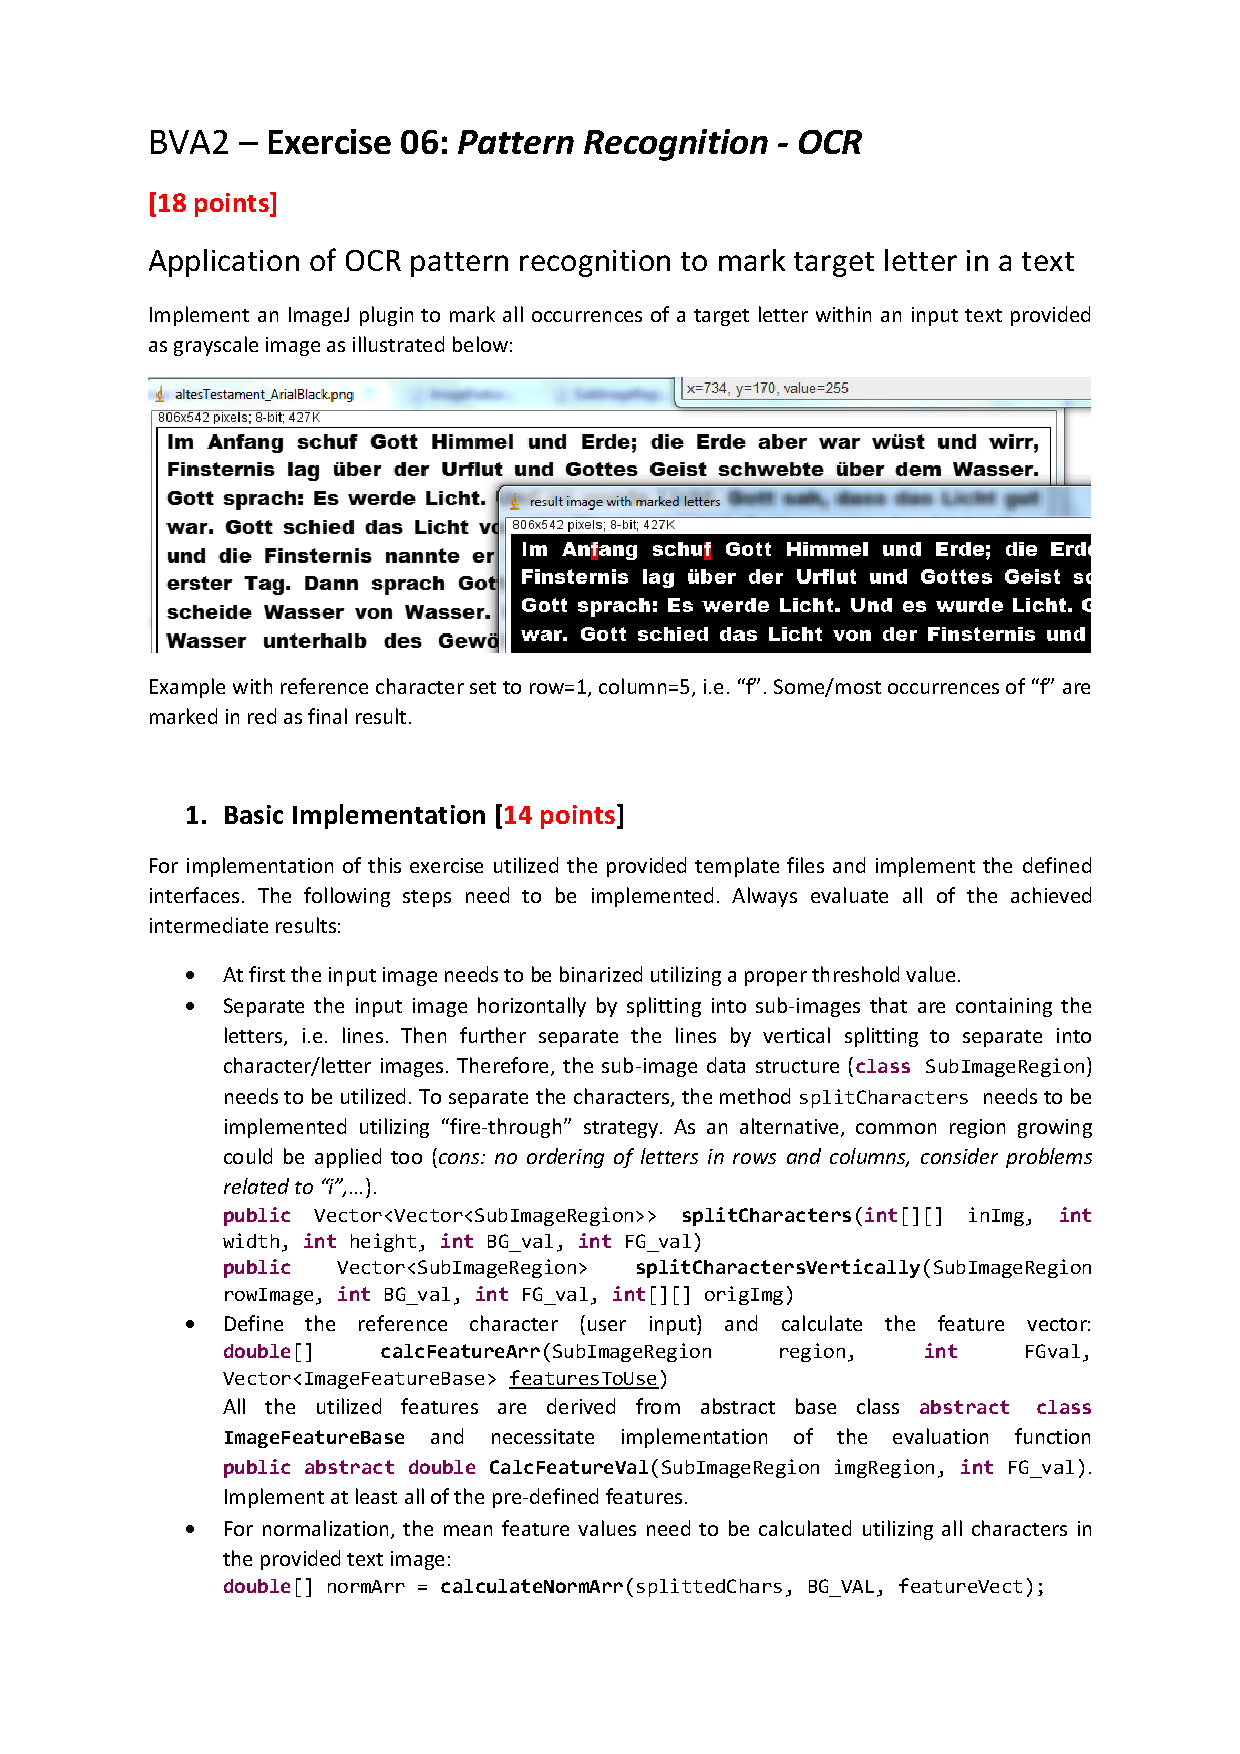
\includepdf[pages={1,2}]{Angabe.pdf}


\section{Basic Implementation}
\subsection{Lösungsidee}
\begin{itemize}
	

\item \textbf{splitCharacters(int[][] InImg, int width, int height, int BG\_val, int FG\_val): }
In dieser Methode werden Zeilen erkannt. Solang eine Reihe rein aus BG\_val besteht, wird diese nicht in das SubImage mitaufgenommen. Sobald nun eine Zeile mit mindestens einem FG\_val kommt, wird diese als Startpunkt des SubImage markiert. Solang nun keine Reihe mit rein aus BG\_val bestehenden Pixeln kommt, wird fortgefahren.
Kommt nun eine Zeile mit lediglich BG\_val, endet hier das SubImage und es kann im Vector gespeichert werden. Dieser Vorgang wird solange wiederholt, bis das Ende des Images erreicht ist.

\item \textbf{splitCharactersVertically(int[][] InImg, int width, int height, int BG\_val, int FG\_val): }
Diese Methode wird ähnlich zur vorherigen implementiert. Es wird lediglich das Durchlaufen des Bildes auf spaltenweise geändert.

\item \textbf{calcFeatureArr(SubImageRegion region, int FGval, Vector$<$ImageFeatureBase$>$ featuresToUse: }
Hier wird für die angegebene SubImageRegion jeder Feature-Wert der angegebenen Features berechnet. Dies wird über die Methode \textit{CalcFeatureVal} berechnet, die jedes Feature implementieren muss.

\item \textbf{calculateNormArr(splittedChars, BG\_VAL, featureVect): }
In dieser Methode wird für jedes Feature der Mittelwert aller SubImages ausgerechnet. Dies dient zum Normalisieren, da sonst höhere Werte bevorzugt werden.
\end{itemize}
\subsubsection{Features}

\begin{itemize}
	\item \textbf{F1: number of pixels: }
	Bei diesem Feature werden die Anzahl an FG\_val-gefärbten Pixel im SubImage berechnet.
	
	\item \textbf{F2: extent in x-direction (max width): } 
	Hier wird die maximale Anzahl an FG\_val Pixel einer Reihe berechnet. Dazu wird eine Counter-Variable definiert.
	
	\item \textbf{F3: extent in y-direction (max height): }
	Hier wird die maximale Anzahl an FG\_val Pixel einer Spalte berechnet. Dazu wird eine Counter-Variable definiert.
	
	\item \textbf{F4: average distance from centroid: } Zuerst wird die Berechnung des Zentroide in einer eigenen Hilfsfunktion implementiert, welche später auch für die restlichen Features (die den Zentroiden benötigen) verwendet werden kann. Die X-Koordinate des Zentroiden wird bestimmt, indem alle X-Koordinaten der Pixel, die zum jeweiligen Buchstaben gehören, aufsummiert werden und durch die Anzahl der beteiligten Pixel dividiert werden. Für die Y-Koordinate werden dann die jeweiligen y-Koordinaten aufsummiert. 
	Um die durchschnittliche Distanz zum Zentroiden zu berechnen werden alle Distanzen zu allen Pixeln die zum Buchstaben gehören aufsummiert und durch die Anzahl der Pixel geteilit. Zum bestimmen der Distanz wird die Formel $\sqrt{((x\textsubscript{2} - x\textsubscript{1})^2 + (y\textsubscript{2} - y\textsubscript{1})^2)}$ verwendet.
	
	\item \textbf{F5: min distance from centroid: } Um die minimale Distanz zum Zentroiden zu bestimmen wird der Zentroide wieder mit der zuvor implementierten Hilfsfunktion bestimmt, um dann die minimale Distanz zu finden.
	
	\item \textbf{F6: max distance from centroid: } Funktioniert gleich wie das Bestimmen der minimalen Distanz, nur das hier die maximale Distanz als Ergebnis gespeichert wird.
	
	\item \textbf{F7: circularity: } Zur Berechnung der \enquote{Circularity} wirde folgende Formel herangezogen:\\ $circularity = \frac{4\pi * area}{perimeter^2}$. Wobei \enquote{area} die Anzahl der Pixel eines Zeichens und \enquote{perimeter} die Anzahl der Pixel des Umfangs sind. Beide Werte können über die ImageJ-Klasse \enquote{Analyzer} ermittelt werden.
	
	\item \textbf{F8: rel pos centroid within bounding box, x-direction: } Zur Berechnung des Zentroiden kann wieder die Hilfsfunktion von vorher verwendet werden. Danach kann die relative Position in x-Richtung berechnet werden.
	
	\item \textbf{F9: rel pos centroid within bounding box, y-direction: } Funktioniert Äquivalent zu F8, nur das hier die Position in y-Richtung berechnet wird.
	
\end{itemize}

\subsection{Fragen}
\begin{itemize}
\item \textbf{Which letters can be detected in a confident way and which letters lead to problems - and why?}
%TODO

\item \textbf{Are all fonts applicable to this kind of OCR strategy - why or why not?: }
Nein, diese Strategie ist nicht mit allen Schriften möglich. Bei z.B. Schreibschriften oder Schriften, wo durchgehende Übergänge zwischen den Buchstaben sind, ist die Separierung der einzelnen Buchstaben nicht möglich. Auch bei handgeschriebene Buchstaben, wo dieselben Zeichen unterschiedlich aussehen (durch Handschrift), ist die Erkennung nicht exakt möglich.

\item \textbf{Does classification accuracy depend on the other characters in the specific line - if that's the case: why and how to overcome this issue?}
Ja, da z.B. ein i, wenn in der Zeile ein g vorhanden ist, eine größere Bounding-Box aufweist, als ein i, wenn in der Zeile kein g vorhanden ist.
Dies kann bei der Berechnung der Features Probleme bereiten, da das SubImage bei beiden i's nicht ident ist.
Man könnte z.B. jedes SubImage selbst noch einmal \glqq zuschneiden\grqq{} und so die restlichen leeren Zeilen wegschneiden.
\end{itemize}

\subsection{Ausarbeitung}
\begin{code}
	\caption{OCRanalysis\_.java}
	\javaFile{\srcDir/OCRanalysis_.java}
	\label{src:exercise-OCRanalysis-java}
\end{code}

\subsection{Tests}

\end{document}